Do wykonania projektu został wykorzystany zewnętrzny układ z mikrofonem. Schemat tego układu jest przedstawiony na rys. \ref{uklad}.
\begin{figure}
    \label{uklad}
    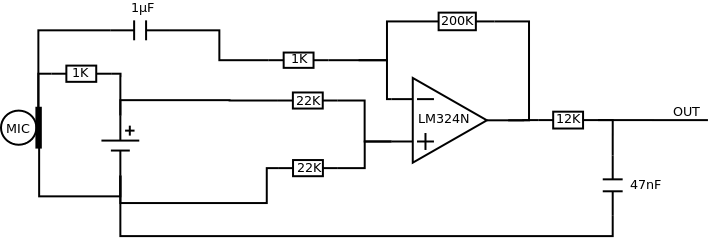
\includegraphics[width=1.0\textwidth]{schemat_mic.png}
    \caption{Schemat układu z mikrofonem}
\end{figure}
Układ jest zasilany z tego samego źródła co mikrokontroler, czyli 3.3V. Główną funkcję pełnią mikrofon, który generuje zmienny sygnał odpowiadający częstotliwości drgań powietrza i wzmacniacz operacyjny, który wzmacnia powstały sygnał 200 razy. Wyjście OUT jest bezpośrednio połączone z wejściem ADC mikrokontrolera.
